\section{Flyback}

The flyback converter is another option for a DC-DC converter. It comes with galvanic isolation between the input and outputs. The flyback converter is basically a buck-boost converter, but here the inductor is split to form a transformer. The windings of the transformer can have different turns ratio and in that way it is possible to step the voltage and current both up or down. 

The basic circuit of the topology can be seen in figure \ref{Flyback_SCHEMATIC}. It uses a switch, a diode and a single control device.    

\begin{figure}[htbp]
	\begin{center}
	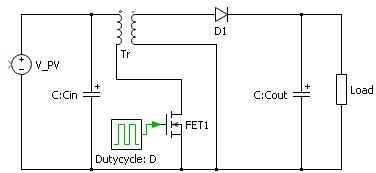
\includegraphics[width=0.7\textwidth]{../Pictures/flyback_schem.png}
	\caption{Flyback converter}
	\label{Flyback_SCHEMATIC}
	\end{center}
\end{figure}

When the MOSFET is on, the energy is transferred from the input voltage source to the transformer. In this state the output capacitor will supply the load with the output voltage. In the off-state the transformer will supply the output load with energy while it charges the capacitor as well. \cite{wiki}

Because of the single control device another advantage of the flyback converter is a wide choice of controllers. For example it is possible to directly connect a PWM controlled IC to control the MOSFET, and by that the converter. 

The drawbacks are primary the current and voltage waveforms. The stress on the switch and diode can be high and comes as a function of the turns ratio of the transformer. Furthermore the leakage inductance from the transformer will result in a big voltage spike at the rising edge of the MOSFET. This needs to be reduced by a snubber circuit. This will increase the power loss and efficiency though. The leakage inductance will also produce transients which will make the voltage stress at the FET bigger and give high-frequency ringing at the input. Lastly there will be increased noise at both terminals due to the fact that the input and output currents are discontinous. 

"Non inverting buckboost texasConverter"
